

\section{Future Directions and Challenges}

\subsection{Future Direction}

The launch of WAAS (Web3 as a Service) marks a transformative leap in bridging the gap between Web2 and Web3 by enabling seamless integration through the Omnichain Web. As businesses, governments, and institutions seek to harness the power of decentralized technologies, WAAS provides a secure and scalable framework to connect their existing systems with the Web3 ecosystem. By leveraging the ZK Adapter and ZK Client, WAAS facilitates trustless interactions across multiple Layer 1 (L1) and Layer 2 (L2) blockchains, as well as rollups, ensuring interoperability without compromising security. This allows enterprises to efficiently manage critical operations such as deposits, withdrawals, contract interactions, and address management—all without relying on centralized intermediaries. With WAAS, Web2 entities can seamlessly onboard into Web3, unlocking new possibilities in a decentralized and interconnected digital landscape.

By offering omnichain capabilities, WAAS extends its reach beyond single-chain ecosystems, empowering Web2 entities, traditional institutions, governments, and banks to create their own decentralized operations. The ability to seamlessly connect with the entire Web3 space, while maintaining the security and trustlessness inherent in blockchain technology, is set to unlock new possibilities for innovation across industries. These advancements pave the way for a more inclusive and decentralized future, where organizations can access the power of blockchain without compromising security or scalability.

WAAS is poised to revolutionize the way companies engage with decentralized technologies, offering an efficient, transparent, and autonomous approach to cross-chain interactions. By enabling decentralized applications (dApps) and services to span across various blockchains, it fosters a new paradigm of collaboration and innovation, pushing the boundaries of what is possible in both Web2 and Web3 spaces. As a result, WAAS will play a key role in the ongoing development of decentralized finance (DeFi), supply chain management, identity systems, and beyond.

\subsubsection{Use Case: Existing L2's}
The ZK adapter plays a crucial role in transforming existing Layer 2 (L2) chains into fully omnichain ecosystems by enabling seamless cross-chain interoperability. Traditionally, L2 chains operate within isolated environments, limiting their ability to interact efficiently with other blockchains. By integrating the ZK Adapter, these chains gain the capability to verify and process cross-chain transactions in a secure, scalable, and trustless manner. The adapter leverages zero-knowledge proofs (ZKPs) to validate transactions across different blockchains without revealing sensitive information, ensuring both privacy and efficiency. Through this mechanism, all cross-chain transactions are routed through the Omnichain Web, a unified framework that standardizes communication between blockchains. This allows L2 networks to interact with multiple Layer 1 (L1) and L2 chains, as well as rollups, without requiring extensive protocol modifications or centralized intermediaries. As a result, L2 chains become inherently Omnichain, gaining access to a broader liquidity pool, improved composability, and greater adoption while maintaining their native security and scalability advantages.

\begin{figure}[h]
    \centering
    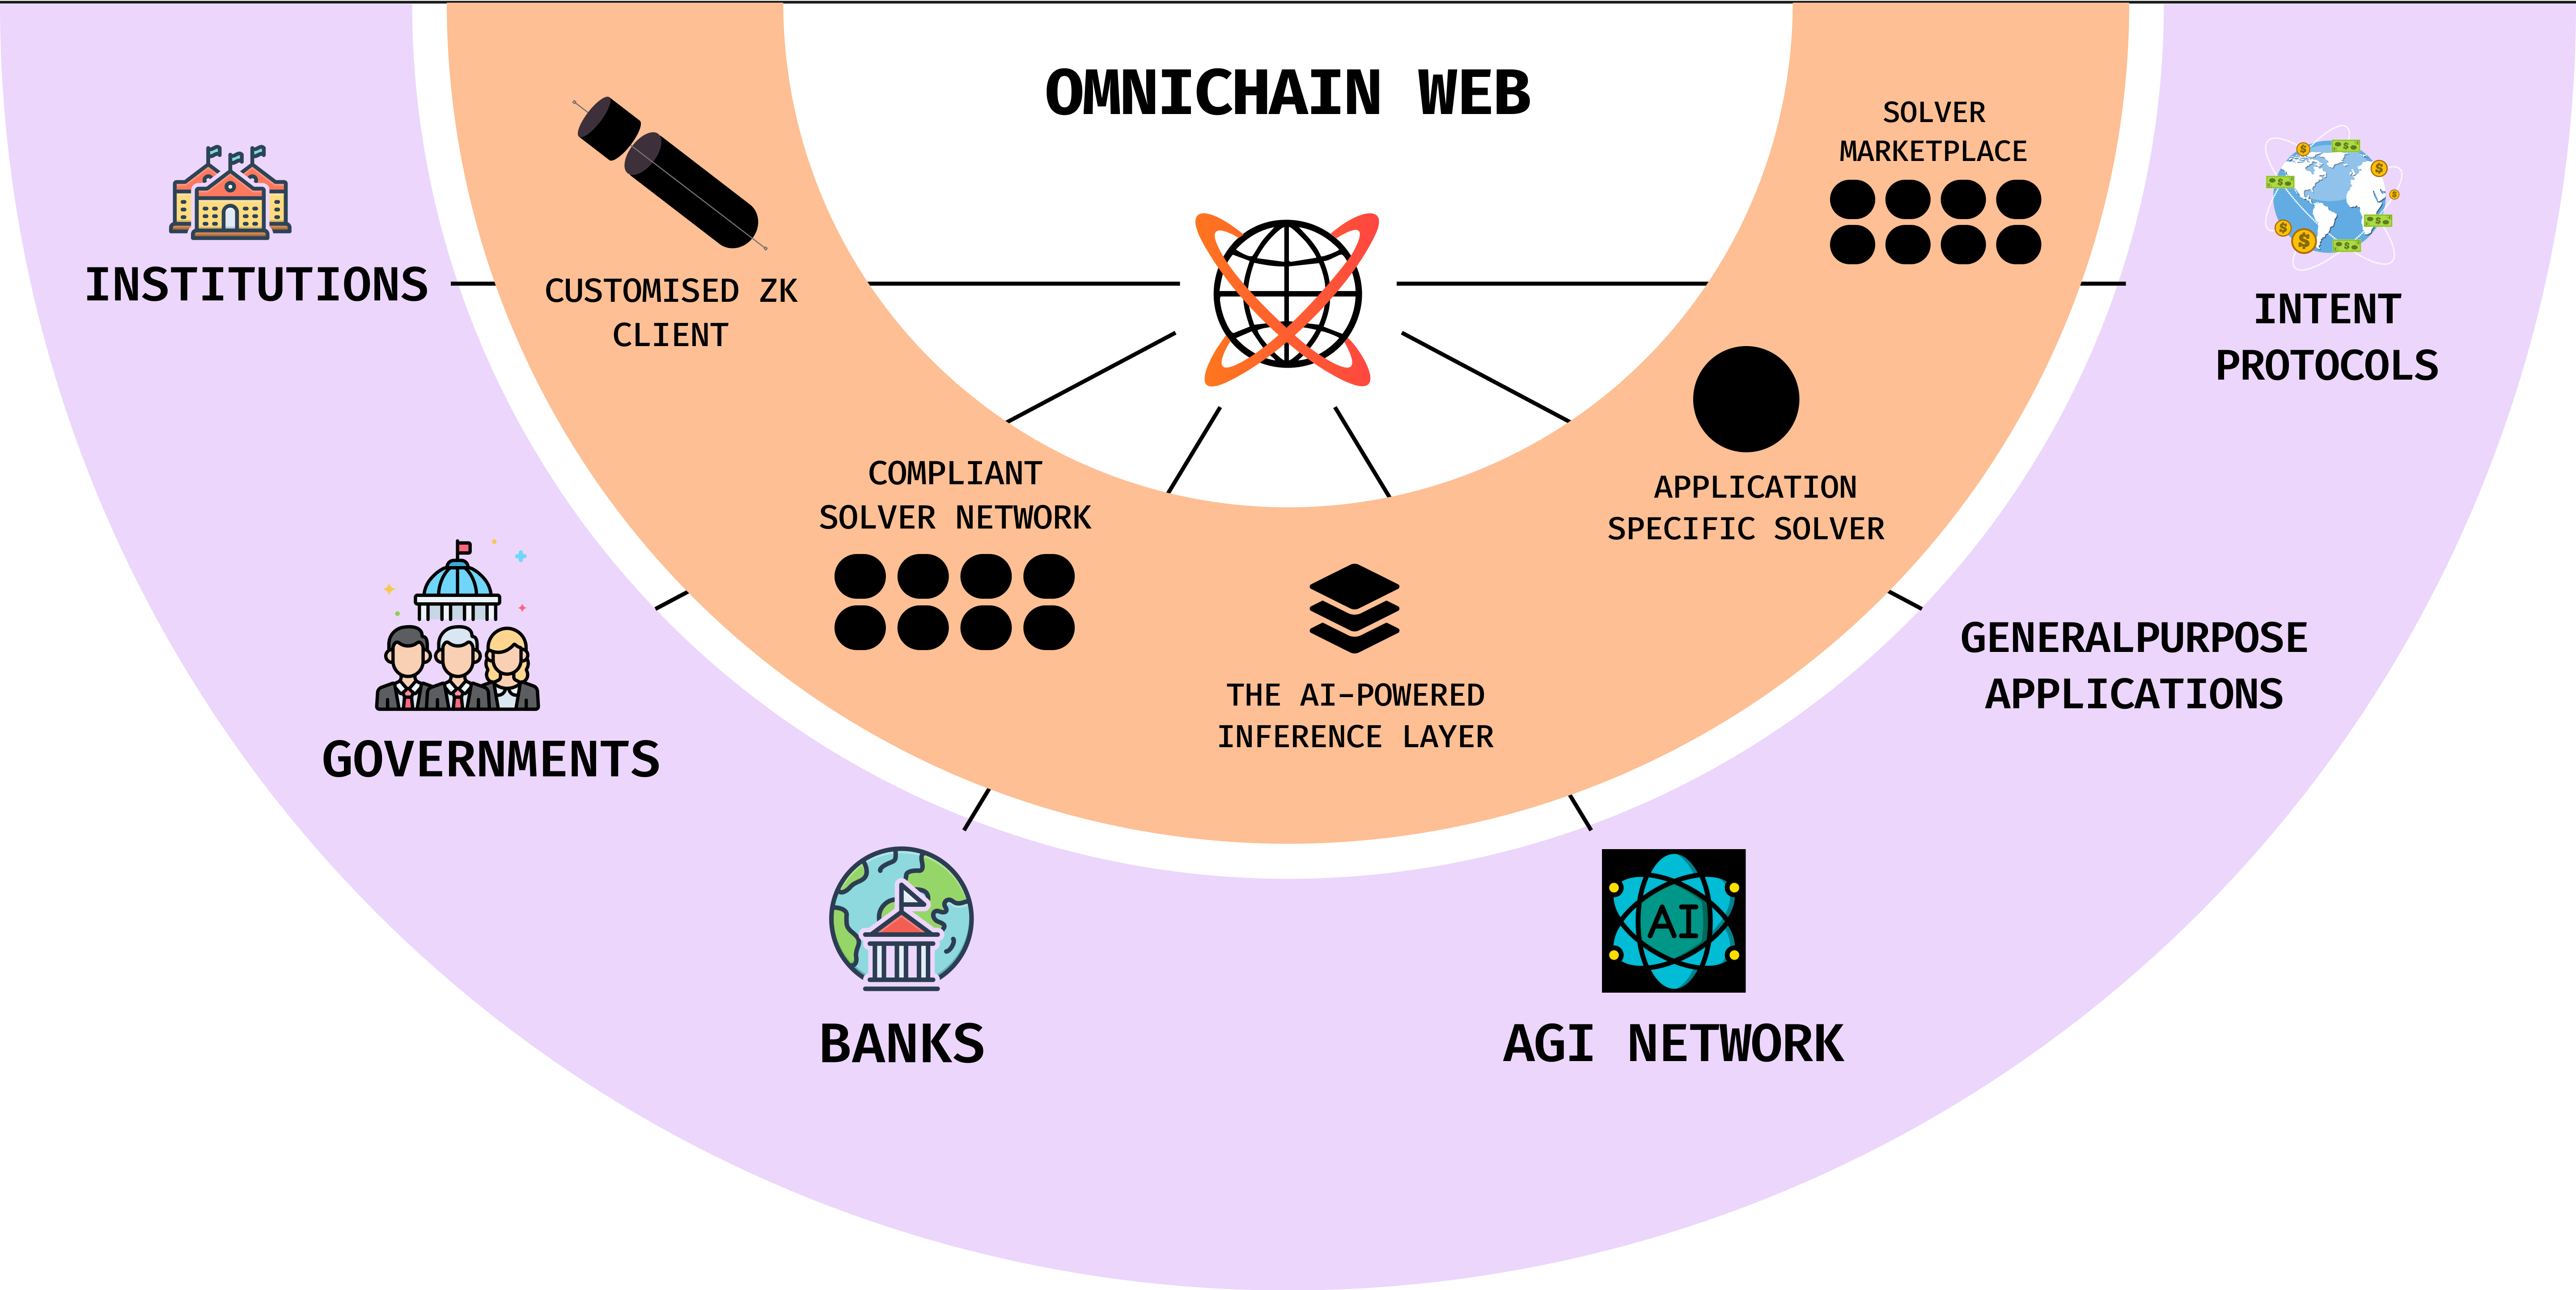
\includegraphics[width=0.9\linewidth]{figure/future.png}
    \caption{Mainstream Expansion}
    \label{fig:solver}
\end{figure}

\subsubsection{Use Cases: Bridging Web2 and Web3}

Currently, Web2 and traditional finance processes an astounding 6.7 billion transactions every day, but Web3 captures less than 1\% of this potential—a significant gap that highlights the scale of opportunity and the hurdles facing Web3 adoption. The next major opportunity lies in connecting Web2's vast scale with Web3's decentralized infrastructure. WAAS enables businesses and institutions to tap into the transformative power of blockchain technology without needing to overhaul their legacy systems. Following are some of the usecases.
 
\begin{itemize}
    \item Government and Public Sector Governments can use WAAS to integrate blockchain technology into public services such as voting, land registry, and identity management. With decentralized identity systems powered by Web3, governments can manage citizen data securely and privately without relying on centralized databases. Cross-chain interoperability ensures that these systems can interact with various blockchains to facilitate secure data transfer, ensuring broader adoption and improved efficiency. A government may also use WAAS to implement a decentralized voting system where voter identities are verified on a blockchain, ensuring transparency and security without relying on intermediaries.

    \item Financial Institutions and Banks Traditional banks are under increasing pressure to adapt to decentralized finance (DeFi). WAAS enables financial institutions to interact with multiple Layer 1 (L1) and Layer 2 (L2) blockchains, facilitating cross-chain transactions for activities such as cross-border payments, asset management, and decentralized lending platforms. By connecting Web2’s scale with Web3’s infrastructure, WAAS helps banks tap into the vast potential of Web3 without overhauling their existing systems. A bank using WAAS can offer customers seamless cross-border payments that utilize the most efficient blockchain, reducing fees and increasing transaction speed while maintaining compliance with regulatory standards.

    \item Institutions and Enterprises Enterprises looking to adopt blockchain for supply chain management, contract validation, or asset tracking can leverage WAAS to integrate Web3 solutions into their existing Web2 systems. WAAS ensures secure and scalable interactions between their traditional platforms and decentralized systems, offering the ability to track goods and services through immutable ledgers across multiple blockchains. A supply chain company could use WAAS to track products in real-time across multiple jurisdictions using blockchain, ensuring that all transactions (e.g., product movements, payments) are validated and traceable without the need for intermediaries.

    \item General-Purpose Applications Any general-purpose application, from social media platforms to gaming networks, can utilize WAAS to add decentralized features while maintaining their traditional user base. For instance, developers can create decentralized applications (dApps) that allow users to transfer assets, verify identities, or interact with smart contracts across multiple blockchains—all while ensuring the ease and familiarity of Web2 experiences. A gaming platform can leverage WAAS to integrate decentralized ownership of in-game assets, where players can buy, sell, and trade assets across various blockchain networks without losing the usability and performance of the platform.
\end{itemize}


By enabling cross-chain interactions, WAAS makes it possible for entities to securely and efficiently interact across various blockchain platforms, ensuring that they can participate in the Web3 ecosystem while benefiting from its scalability, security, and decentralization. As more industries explore the possibilities of Web3, WAAS will play a pivotal role in accelerating the adoption of blockchain technologies, helping to bridge the gap between today’s Web2-driven world and the decentralized future of Web3.

\subsection{Challenges}

Despite its immense potential, the deployment and adoption of WAAS face several significant challenges that need to be addressed as part of its continued evolution.

\begin{itemize}
    \item[1.] \textbf{Scalability and Performance in zk Systems}
    
   While the ZK adapter and the ZK client improve security, scalability remains a fundamental concern in the zk verification system.  Efficiently scaling WAAS to handle large-scale deployments while maintaining low latency and high throughput across different blockchains will require ongoing research and optimization of both the ZK protocols and the underlying infrastructure.

   \item[2.] \textbf{Regulatory and Legal Compliance}
   
   The decentralized and trustless nature of Web3 introduces complexities when it comes to regulatory compliance, especially for traditional institutions such as banks and governments. Navigating the rapidly changing landscape of blockchain regulation, including issues related to data privacy, anti-money laundering (AML), and know-your-customer (KYC) requirements, will be critical. WAAS must find ways to enable decentralized operations while complying with these regulations, ensuring that Web3 integrations do not conflict with existing legal frameworks.

    \item[3.] \textbf{Adoption and Education}
    
   One of the key challenges for WAAS will be adoption by Web2 companies and traditional institutions. Many of these organizations have limited experience with decentralized technologies and may be hesitant to adopt Web3 solutions due to perceived complexity or lack of understanding. WAAS will need to offer easy-to-use tools, comprehensive support, and educational resources to help these entities make the transition to decentralized operations smoothly. Convincing these organizations of the tangible benefits—such as cost savings, enhanced security, and greater efficiency—of integrating with Web3 will require a concerted effort in demonstrating value and fostering trust in the system.
\end{itemize}


\subsection{Conclusion}


The Omnichain Web is set to transform decentralized technology by addressing critical challenges in cross-chain interoperability, liquidity fragmentation, execution efficiency, and capital flow management. Through the integration of omnichain rollups, cross-chain intent standardization, and a decentralized solver network, this architecture eliminates inefficiencies, optimizes liquidity utilization, and provides a unified framework for seamless execution across multiple L1 and L2 ecosystems.  

One of the most pressing issues in Web3 has been fragmented liquidity and execution inefficiencies across chains. The Omnichain Web solves this by enabling peer-to-peer liquidity rebalancing, reducing reliance on centralized bridges that are often prone to security vulnerabilities. Additionally, the solver network, powered by omni-rollups, ensures efficient cross-chain intent fulfillment by netting complementary transactions, thereby minimizing capital inefficiencies and enhancing execution speed.  

Furthermore, the adoption of Dynamic Threshold Signature Scheme (TSS) enhances security by eliminating single points of failure in multi-party signing. Unlike static TSS, which requires pre-configured key shares, dynamic TSS allows flexible participation in signing operations, enabling more robust validator and solver rotation while maintaining decentralized security guarantees.  

The Ragno Network plays a pivotal role in enabling secure, scalable, and decentralized state management within the Omnichain Web. By ensuring deterministic state synchronization across omnichain rollups, Ragno provides a consistent execution environment where solvers can efficiently process intents, manage liquidity, and rebalance capital across various blockchains. This eliminates settlement risks and ensures trust-minimized execution, making cross-chain transactions more efficient and secure.  

  
Looking ahead, the Omnichain Web aims to enhance solver network capabilities by integrating AI-driven solvers for optimal liquidity management and efficient intent execution. Additionally, it seeks to develop regulatory-friendly solutions tailored for enterprises, institutions, and governments through its Web3-as-a-Service (WAAS) offerings. By eliminating inefficiencies in blockchain interoperability and enabling seamless cross-chain interactions, the Omnichain Web is positioned to become the foundation of the next-generation Web3 economy, effectively bridging the gap between Web2 and Web3 in a scalable and sustainable way.